\documentclass{beamer}
\usetheme{Madrid}
\usecolortheme{beaver}
\usepackage{tikz}
\usepackage{booktabs}
\usetikzlibrary{shapes}

\title{Introduction to Bullshit: From Philosophy to Practice}
\subtitle{A Critical Thinking Journey}
\author{Brendan Shea, PhD}
\date{Intro to Logic}

\begin{document}
	
	\frame{\titlepage}
	
	% Slide 1: What Is Bullshit? An Introduction to a Philosophical Problem
	\begin{frame}{What Is Bullshit? An Introduction to a Philosophical Problem}
		\begin{itemize}
			\item \textbf{Bullshit} is a distinct form of communication that differs from both truth-telling and lying in important ways.
			\item Unlike a liar who knows the truth and deliberately says something false, a bullshitter shows complete indifference to whether their statements are true or false.
			\item The philosophical study of bullshit helps us understand how language can be used to manipulate and obscure rather than communicate.
			\item Recognizing bullshit is a crucial skill in our information-rich world where not all speech aims at truth.
		\end{itemize}
		
		\begin{alertblock}{Key Insight}
			Bullshit is more dangerous than lies because it erodes our very concern for truth.
		\end{alertblock}
	\end{frame}
	
	% Slide 2: Why Study Bullshit in a Logic Class?
	\begin{frame}{Why Study Bullshit in a Logic Class?}
		\begin{itemize}
			\item Logic teaches us to evaluate arguments based on their structure and the truth of their premises, but bullshit operates outside this framework.
			\item Understanding bullshit strengthens our \textbf{critical thinking} skills by teaching us to recognize when someone isn't even trying to make valid arguments.
			\item In a world full of social media, AI-generated content, and political rhetoric, the ability to detect bullshit has become essential for informed citizenship.
			\item Studying bullshit connects abstract logical principles to real-world communication challenges you face every day.
		\end{itemize}
		
		\begin{block}{Connection to Logic}
			Traditional logic assumes speakers aim for truth. Bullshit analysis examines what happens when this assumption breaks down.
		\end{block}
	\end{frame}
	
	% Slide 3: Course Overview: From Theory to Real-World Applications
	\begin{frame}{Overview: From Theory to Real-World Applications}
		\begin{itemize}
			\item We'll begin with philosopher Harry Frankfurt's groundbreaking theory that defines bullshit as speech unconcerned with truth or falsity.
			\item Next, we'll examine how social media platforms create perfect conditions for bullshit to thrive and spread rapidly.
			\item We'll then explore how artificial intelligence can generate plausible-sounding but potentially meaningless or false content at unprecedented scale.
			\item Finally, we'll analyze how political bullshit, especially from populist movements, can threaten the shared reality necessary for democratic deliberation.
		\end{itemize}
		
		\begin{block}{What we'll cover}
			\begin{enumerate}
				\item Frankfurt's philosophical framework
				\item Social media case studies
				\item AI and synthetic content
				\item Political applications and democracy
			\end{enumerate}
		\end{block}
	\end{frame}
	
	% Slide 4: Harry Frankfurt: The Philosopher Who Defined Bullshit
	\begin{frame}{Harry Frankfurt: The Philosopher Who Defined Bullshit}
		\begin{itemize}
			\item Harry Frankfurt is a distinguished philosopher at Princeton University who spent most of his career studying free will, personal identity, and moral responsibility.
			\item In 1986, he published a short essay called "On Bullshit" that became his most famous work, later republished as a bestselling book in 2005.
			\item Frankfurt argued that bullshit deserved serious philosophical analysis because it represents a unique and dangerous form of dishonesty.
			\item His work transformed bullshit from a vulgar term into a \textbf{technical concept} in philosophy, communication studies, and critical thinking.
		\end{itemize}
		
		\begin{block}{Frankfurt's Contribution}
			"One of the most salient features of our culture is that there is so much bullshit. Everyone knows this." - Opening line of "On Bullshit"
		\end{block}
	\end{frame}
	
	% Slide 5: "On Bullshit": The Essay That Started It All
	\begin{frame}{"On Bullshit": The Essay That Started It All}
		\begin{itemize}
			\item Frankfurt's essay begins by noting that despite bullshit's prevalence in our culture, we lack a clear understanding of what it actually is.
			\item He argues that \textbf{bullshit} is not merely casual talk or hot air, but a specific form of deceptive communication with its own characteristics.
			\item The essay uses philosophical analysis to distinguish bullshit from related concepts like lying, bluffing, and mere carelessness with facts.
			\item Frankfurt's central thesis is that the \textbf{essence of bullshit} is a complete lack of concern for how things really are—an indifference to truth itself.
		\end{itemize}
		
		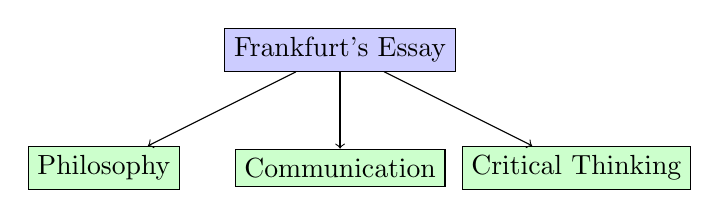
\begin{tikzpicture}
			\node[draw, rectangle, fill=blue!20] (essay) at (0,0) {Frankfurt's Essay};
			\node[draw, rectangle, fill=green!20] (phil) at (-3,-1.5) {Philosophy};
			\node[draw, rectangle, fill=green!20] (comm) at (0,-1.5) {Communication};
			\node[draw, rectangle, fill=green!20] (crit) at (3,-1.5) {Critical Thinking};
			\draw[->] (essay) -- (phil);
			\draw[->] (essay) -- (comm);
			\draw[->] (essay) -- (crit);
		\end{tikzpicture}
	\end{frame}
	
	% Slide 6: Truth, Lies, and the Space Between
	\begin{frame}{Truth, Lies, and the Space Between}
		\begin{itemize}
			\item When someone tells the \textbf{truth}, they attempt to describe reality accurately based on their genuine beliefs about how things are.
			\item When someone tells a \textbf{lie}, they know what is true but deliberately assert something false to deceive their audience.
			\item \textbf{Bullshit} occupies a third space: the speaker neither knows nor cares whether their statements correspond to reality.
			\item This indifference to truth makes bullshit fundamentally different from both honest mistakes and calculated deceptions.
		\end{itemize}
		
		\begin{table}
			\begin{tabular}{lcc}
				\toprule
				\textbf{Type} & \textbf{Knows Truth?} & \textbf{Cares About Truth?} \\
				\midrule
				Truth-teller & Yes/Tries to & Yes \\
				Liar & Yes & Yes (to violate) \\
				Bullshitter & No/Maybe & No \\
				\bottomrule
			\end{tabular}
		\end{table}
	\end{frame}
	
	% Slide 7: The Bullshitter's Relationship to Truth
	\begin{frame}{The Bullshitter's Relationship to Truth}
		\begin{itemize}
			\item The bullshitter's \textbf{indifference to truth} is what makes bullshit uniquely corrosive to honest discourse and rational deliberation.
			\item While a liar must pay attention to the truth in order to conceal it effectively, a bullshitter ignores the truth entirely.
			\item Bullshitters may sometimes say true things and sometimes say false things, but truth or falsity is never their goal or concern.
			\item This disconnection from truth-seeking makes bullshit more dangerous than lying because it attacks the very enterprise of trying to establish what is real.
		\end{itemize}
		
		\begin{alertblock}{Frankfurt's Warning}
			The bullshitter "does not care whether the things he says describe reality correctly. He just picks them out, or makes them up, to suit his purpose."
		\end{alertblock}
	\end{frame}
	
	% Slide 8: Indifference vs. Deception: The Key Distinction
	\begin{frame}{Indifference vs. Deception: The Key Distinction}
		\begin{itemize}
			\item \textbf{Deception} requires the deceiver to have a specific false belief they want their audience to adopt, which means they must track what is actually true.
			\item \textbf{Indifference} means the speaker doesn't care whether their audience's resulting beliefs are true or false—only that they achieve some other goal.
			\item A liar says "It's sunny outside" knowing it's raining because they want you to leave without an umbrella, while a bullshitter might say the same thing without even checking the weather.
			\item This distinction explains why fact-checking often fails against bullshit: the bullshitter isn't trying to avoid being caught in falsehoods.
		\end{itemize}
		
		\begin{example}
			\textbf{Liar}: "I have a PhD from Harvard" (knows they don't)\\
			\textbf{Bullshitter}: "A Harvard professor said..." (doesn't care whether this is true)
		\end{example}
	\end{frame}
	
	% Slide 9: Why Bullshit Might Be Worse Than Lying
	\begin{frame}{Why Bullshit Might Be Worse Than Lying}
		\begin{itemize}
			\item Frankfurt argues that \textbf{bullshit poses a greater threat} to truth than lying because it undermines the very concept that truth matters.
			\item Each lie is a localized assault on truth about a specific fact, while bullshit erodes the general habit of caring whether our statements correspond to reality.
			\item When bullshit becomes normalized, people stop expecting speakers to even attempt accuracy, which destroys the foundation of rational discourse.
			\item A culture saturated with bullshit loses the shared commitment to truth that makes productive disagreement and learning possible.
		\end{itemize}
		
		\begin{alertblock}{The Greater Danger}
			\begin{itemize}
				\item \textbf{Lies}: Attack specific truths
				\item \textbf{Bullshit}: Attacks the value of truth itself
				\item \textbf{Result}: Epistemic nihilism—nothing matters
			\end{itemize}
		\end{alertblock}
	\end{frame}
	
	% Slide 10: The Bullshitter's Goals: Impression Over Accuracy
	\begin{frame}{The Bullshitter's Goals: Impression Over Accuracy}
		\begin{itemize}
			\item The bullshitter's primary goal is to create a certain \textbf{impression of themselves} rather than to communicate information about the world.
			\item Common bullshitter goals include appearing knowledgeable, seeming important, avoiding blame, or filling awkward silence with confident-sounding words.
			\item A job applicant who claims expertise in "quantum blockchain synergy" isn't trying to deceive about a real skill—they're trying to sound technically sophisticated.
			\item This focus on \textbf{impression management} explains why bullshitters often use vague buzzwords, complex jargon, and unfalsifiable claims.
		\end{itemize}
		
		\begin{block}{Classic Bullshit Phrases}
			\begin{tabular}{ll}
				"Studies show..." & (which studies?) \\
				"Everyone knows..." & (who exactly?) \\
				"It's common sense..." & (is it though?) \\
				"Trust me..." & (based on what?) \\
			\end{tabular}
		\end{block}
	\end{frame}
	
	% Slide 11: Frankfurt's Examples: From Art to Politics  
	\begin{frame}{Frankfurt's Examples: From Art to Politics}
		\begin{itemize}
			\item Frankfurt illustrates bullshit with the example of a Fourth of July orator who makes grand pronouncements about patriotism without caring if they're true.
			\item He discusses how \textbf{bull sessions}—casual conversations where people try out ideas without commitment—can slide into bullshit when speakers pretend their musings are serious claims.
			\item In art and advertising, bullshitters make sweeping statements about products or artworks ("This painting captures the essence of humanity") without concern for accuracy.
		\end{itemize}
		
		\begin{example}
			\scriptsize
			\textbf{Fourth of July Orator}: "Our founding fathers would be proud of how we've fulfilled their vision!"
			\begin{itemize}
				\item Never studied what the founders actually wanted
				\item Doesn't care if statement is historically accurate  
				\item Only cares that audience feels patriotic
			\end{itemize}
		\end{example}
	\end{frame}
	

	% Slide 13: The Perfect Storm: Why Social Media Breeds Bullshit
	\begin{frame}{The Perfect Storm: Why Social Media Breeds Bullshit}
		\begin{itemize}
			\item Social media platforms create ideal conditions for bullshit by rewarding \textbf{engagement} (likes, shares, comments) rather than accuracy or truth.
			\item The pressure to post constantly means users often share content without checking facts, embodying Frankfurt's "indifference to truth."
			\item The \textbf{viral nature} of social media means bullshit can spread to millions before any fact-checking occurs, if it ever does.
			\item Platform algorithms amplify emotionally provocative content regardless of accuracy, giving bullshit a systematic advantage over careful, truthful communication.
		\end{itemize}
		
		\begin{alertblock}{The Engagement Trap}
			A false but shocking post gets 10,000 shares. The correction gets 100. Which one shaped more people's beliefs?
		\end{alertblock}
	\end{frame}
	
	% Slide 14: Algorithmic Amplification of Engaging Content
	\begin{frame}{Algorithmic Amplification of Engaging Content}
		\begin{itemize}
			\item Social media \textbf{algorithms} are designed to maximize user engagement by showing content that triggers strong emotional responses.
			\item These algorithms don't evaluate truth or falsity—they only measure clicks, time spent, and interactions, perfectly embodying Frankfurt's "indifference to truth."
			\item Bullshit often outperforms truth in engagement metrics because it can be crafted purely to push emotional buttons without the constraints of accuracy.
			\item The result is a \textbf{feedback loop}: successful bullshit gets amplified, teaching content creators that truth is less important than virality.
		\end{itemize}
		
		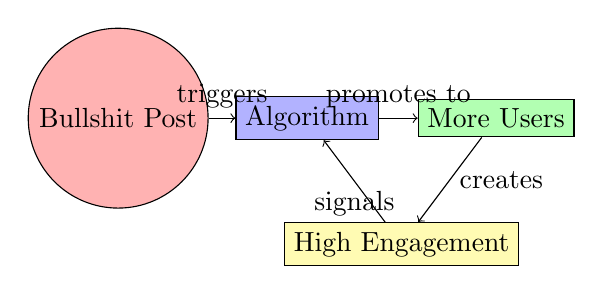
\begin{tikzpicture}[scale=0.8]
			\node[draw, circle, fill=red!30] (bs) at (0,0) {Bullshit Post};
			\node[draw, rectangle, fill=blue!30] (algo) at (3,0) {Algorithm};
			\node[draw, rectangle, fill=green!30] (users) at (6,0) {More Users};
			\node[draw, rectangle, fill=yellow!30] (engage) at (4.5,-2) {High Engagement};
			
			\draw[->] (bs) -- (algo) node[midway, above] {triggers};
			\draw[->] (algo) -- (users) node[midway, above] {promotes to};
			\draw[->] (users) -- (engage) node[midway, right] {creates};
			\draw[->] (engage) -- (algo) node[midway, below] {signals};
		\end{tikzpicture}
	\end{frame}
	
	% Slide 15: The Attention Economy: Clicks Over Truth
	\begin{frame}{The Attention Economy: Clicks Over Truth}
		\begin{itemize}
			\item In the \textbf{attention economy}, human attention is the scarce resource that platforms compete to capture and monetize through advertising.
			\item Content creators learn that provocative bullshit ("Doctors HATE this one trick!") generates more clicks than nuanced truth.
			\item The economic incentives actively discourage fact-checking or careful analysis because these slow down content production and reduce sensationalism.
			\item This system rewards those who are best at crafting engaging bullshit, not those who are most committed to truth or accuracy.
		\end{itemize}
		
		\begin{example}
			\begin{itemize}
				\scriptsize
				\item \textbf{Truth}: "New study shows modest correlation between coffee consumption and alertness in specific conditions"
				\item \textbf{Bullshit}: "Scientists SHOCKED: Coffee is basically a SUPERPOWER!"
				\item Guess which headline gets more clicks?
			\end{itemize}
		\end{example}
	\end{frame}
	
	% Slide 16: Echo Chambers and Confirmation Bias
	\begin{frame}{Echo Chambers and Confirmation Bias}
		\begin{itemize}
			\item \textbf{Echo chambers} form when algorithms show users content similar to what they've already engaged with, creating closed loops of reinforcing beliefs.
			\item Within these chambers, \textbf{confirmation bias} makes people more likely to share content that supports their existing views without checking its accuracy.
			\item Bullshit that aligns with group beliefs spreads unchallenged because the social cost of fact-checking your "team's" claims is higher than going along.
			\item This environment is perfect for bullshitters who can craft messages that feel truthy to specific audiences without any concern for actual truth.
		\end{itemize}
		
		\begin{alertblock}{The Truthiness Problem}
			"Truthiness" (coined by Stephen Colbert): When something feels true based on gut instinct rather than facts. Echo chambers transform bullshit into truthiness.
		\end{alertblock}
	\end{frame}
	
	% Slide 17: Viral Misinformation: Case Studies
	\begin{frame}{Viral Misinformation: Case Studies}
		\begin{itemize}
			\item The "Momo Challenge" hoax spread worldwide through social media, causing panic about a nonexistent threat to children, shared by parents who never verified it.
			\item False health claims about miracle cures spread faster than medical professionals can debunk them because hope and fear are more shareable than careful science.
			\item These cases show how \textbf{emotional resonance} combined with \textbf{indifference to verification} creates perfect conditions for bullshit epidemics.
		\end{itemize}
		
		\begin{example}
			\scriptsize
			\textbf{Anatomy of Viral Bullshit}: The "Dangerous TikTok Trend" Template
			\begin{enumerate}
				\item Claim teens are doing something shocking
				\item Add "Parents need to know!"
				\item Include unverified anecdotes
				\item Watch it spread without anyone checking if the trend actually exists
			\end{enumerate}
		\end{example}
	\end{frame}
	
	% Slide 18: Influencer Culture and Authentic Deception
	\begin{frame}{Influencer Culture and Authentic Deception}
		\begin{itemize}
			\item \textbf{Influencer culture} rewards those who can project an appealing image regardless of whether that image corresponds to reality.
			\item The performance of "authenticity" becomes more important than actual authenticity, creating what we might call \textbf{authentic bullshit}.
			\item Influencers often promote products they've never used or lifestyles they don't actually live, embodying Frankfurt's indifference to truth.
			\item Followers absorb this bullshit because the emotional connection to the influencer overrides critical evaluation of their claims.
		\end{itemize}
		
		\begin{block}{Influencer Bullshit Starter Pack}
			\begin{tabular}{ll}
				"I wake up at 4am every day" & (posted at 2pm) \\
				"This changed my life!" & (sponsored post) \\
				"Just being real with you guys" & (reading from script) \\
				"I've used this for years" & (first time touching product) \\
			\end{tabular}
		\end{block}
	\end{frame}
	
	% Slide 19: The Collapse of Gatekeepers
	\begin{frame}{The Collapse of Gatekeepers}
		\begin{itemize}
			\item Traditional media had \textbf{gatekeepers}—editors, fact-checkers, and journalists—who filtered out at least some bullshit before publication.
			\item Social media eliminated these gatekeepers, allowing anyone to broadcast claims to potentially millions without any verification process.
			\item While democratizing information sounds positive, it also means there's no systematic filter for bullshit before it reaches massive audiences.
			\item The responsibility for detecting bullshit has shifted entirely to individual users who often lack the time, expertise, or motivation to verify claims.
		\end{itemize}
		
		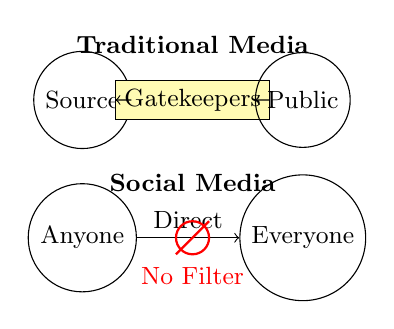
\begin{tikzpicture}[scale=0.7]
			\small
			% Traditional Media
			\node at (0,3) {\textbf{Traditional Media}};
			\node[draw, circle] (source1) at (-2,2) {Source};
			\node[draw, rectangle, fill=yellow!30] (gate1) at (0,2) {Gatekeepers};
			\node[draw, circle] (public1) at (2,2) {Public};
			\draw[->] (source1) -- (gate1);
			\draw[->] (gate1) -- (public1);
			
			% Social Media
			\node at (0,0.5) {\textbf{Social Media}};
			\node[draw, circle] (source2) at (-2,-0.5) {Anyone};
			\node[draw, circle] (public2) at (2,-0.5) {Everyone};
			\draw[->] (source2) -- (public2) node[midway, above] {Direct};
			\draw[red, thick] (0,-0.5) circle (0.3);
			\draw[red, thick] (-0.3,-0.8) -- (0.3,-0.2);
			\node[red] at (0,-1.2) {No Filter};
		\end{tikzpicture}
	\end{frame}
	
	% Slide 20: Digital Literacy: Tools for Detection
	\begin{frame}{Digital Literacy: Tools for Detection}
		\begin{itemize}
			\item \textbf{Digital literacy} means developing skills to navigate online information critically, including recognizing potential bullshit before sharing.
			\item Key detection strategies include checking sources, looking for emotional manipulation, and asking "Who benefits if I believe this?"
			\item The \textbf{SIFT method} (Stop, Investigate the source, Find better coverage, Trace claims) provides a practical framework for evaluating online content.
			\item Remember that bullshitters count on you being too busy or lazy to verify—taking just 30 seconds to check can stop bullshit from spreading.
		\end{itemize}
		
		\begin{block}{Quick Bullshit Detection Checklist}
			\scriptsize
			\begin{enumerate}
				\item Does this seem designed to make me angry or afraid?
				\item Is the source trying to sell me something?
				\item Would I be embarrassed if this turned out to be false?
				\item Can I find this reported by legitimate news sources?
			\end{enumerate}
		\end{block}
	\end{frame}
	
	% Slide 21: Large Language Models: Bullshit Machines?
	\begin{frame}{Large Language Models: Bullshit Machines?}
		\begin{itemize}
			\item \textbf{Large Language Models (LLMs)} like ChatGPT are AI systems trained to produce plausible-sounding text by predicting what words typically follow others.
			\item These models have no conception of truth or falsity—they simply generate text that statistically resembles their training data.
			\item This makes LLMs perfect exemplars of Frankfurt's bullshitter: they are fundamentally \textbf{indifferent to truth} because they have no mechanism for caring about it.
			\item When an AI confidently states facts, it's not lying or telling the truth—it's producing text patterns without any relationship to reality.
		\end{itemize}
		
		\begin{alertblock}{The Fundamental Problem}
			LLMs optimize for plausibility, not truth. They literally cannot tell the difference between accurate information and convincing-sounding nonsense.
		\end{alertblock}
	\end{frame}
	
	% Slide 22: The Hallucination Problem in AI
	\begin{frame}{The Hallucination Problem in AI}
		\begin{itemize}
			\item AI researchers use the term \textbf{hallucination} when models generate false information that sounds completely reasonable and is stated with total confidence.
			\item These aren't mistakes in the traditional sense—the AI isn't misremembering or miscalculating; it's generating plausible-sounding bullshit.
			\item The hallucination problem is inherent to how these models work: they're designed to produce text that fits patterns, not text that corresponds to reality.
		\end{itemize}
		
		\begin{example}
			\scriptsize
			\textbf{Real AI Hallucination Examples:}
			\begin{itemize}
				\item Lawyer used ChatGPT for legal research; it invented entire court cases
				\item Students asked for book summaries; AI created convincing plots for books that never existed
				\item Researchers requested citations; AI generated real-sounding but completely fake papers
			\end{itemize}
		\end{example}
	\end{frame}
	
	% Slide 23: ChatGPT and Confident Incorrectness
	\begin{frame}{ChatGPT and Confident Incorrectness}
		\begin{itemize}
			\item ChatGPT and similar models present all information with the same confident, authoritative tone regardless of accuracy.
			\item This \textbf{uniform confidence} makes it impossible to distinguish between the AI's accurate statements and its complete fabrications.
			\item The model cannot say "I don't know" in any meaningful way—it will always produce something that sounds like an answer.
			\item Users often trust AI responses because they're well-formatted and sound professional, mistaking stylistic competence for factual accuracy.
		\end{itemize}
		
		\begin{block}{The Confidence Game}
			\begin{tabular}{ll}
				\textbf{Human Expert:} & "I think... probably... let me check..." \\
				\textbf{ChatGPT (correct):} & "The answer is definitively X." \\
				\textbf{ChatGPT (hallucinating):} & "The answer is definitively Y." \\
				\multicolumn{2}{l}{Same confidence level, opposite truth values}
			\end{tabular}
		\end{block}
	\end{frame}
	
	% Slide 24: AI-Generated Content: Plausible but False
	\begin{frame}{AI-Generated Content: Plausible but False}
		\begin{itemize}
			\item AI excels at generating content that \textbf{sounds right} because it mimics patterns from millions of real examples in its training data.
			\item This plausibility makes AI-generated bullshit particularly dangerous—it passes our initial "sniff test" for reasonable-sounding information.
			\item AI can produce entire essays, news articles, or scientific abstracts that are structurally perfect but factually meaningless or false.
			\item The sophistication of the bullshit makes it harder to detect than human-generated nonsense, which often contains tell-tale signs of carelessness.
		\end{itemize}
		
		\begin{example}
			\scriptsize
			\textbf{AI-Generated Abstract:}
			"We present a novel framework for quantum-enhanced machine learning using topological insulators. Our results show a 47\% improvement in classification accuracy through non-Abelian anyonic braiding..."
			\begin{itemize}
				\item Sounds impressively technical 
				\item Uses real scientific terms 
				\item Completely meaningless combination 
			\end{itemize}
		\end{example}
	\end{frame}
	
	% Slide 25: Deepfakes and Synthetic Media
	\begin{frame}{Deepfakes and Synthetic Media}
		\begin{itemize}
			\item \textbf{Deepfakes} use AI to create convincing fake videos or audio of real people saying things they never said.
			\item This technology represents bullshit at a new level: not just false claims, but fabricated evidence that seems to support those claims.
			\item The existence of deepfakes creates a \textbf{liar's dividend}—now anyone can dismiss real evidence by claiming it might be AI-generated.
			\item We're entering an era where seeing is no longer believing, making Frankfurt's concern about indifference to truth more urgent than ever.
		\end{itemize}
		
		\begin{alertblock}{The Epistemic Apocalypse}
			When any video could be fake and any fake could look real, how do we establish shared facts about what actually happened?
		\end{alertblock}
	\end{frame}
	
	% Slide 26: The Flood of AI-Generated Text Online
	\begin{frame}{The Flood of AI-Generated Text Online}
		\begin{itemize}
			\item AI tools can generate thousands of articles, reviews, or social media posts per minute, flooding the internet with synthetic content.
			\item This \textbf{bullshit tsunami} makes it increasingly difficult to find genuine human communication or verified information online.
			\item SEO-optimized AI content often ranks higher in search results than carefully researched human-written articles, rewarding bullshit over truth.
			\item Soon, most text online may be AI-generated, creating a "wilderness of mirrors" where detecting authentic human communication becomes nearly impossible.
		\end{itemize}
		
	\end{frame}
	
	% Slide 27: Can AI Detect Its Own Bullshit?
	\begin{frame}{Can AI Detect Its Own Bullshit?}
		\begin{itemize}
			\item Researchers are developing AI systems to detect AI-generated content, but this creates an \textbf{arms race} between generation and detection.
			\item Current detection tools have high error rates and can be fooled by sophisticated AI or flag genuine human writing as artificial.
			\item The fundamental problem remains: if AI doesn't understand truth, how can it identify bullshit based on indifference to truth?
			\item We may need to accept that technical solutions alone cannot solve what is essentially a human problem about our relationship with truth.
		\end{itemize}
		
		\begin{block}{The Detection Paradox}
			\begin{itemize}
				\item AI creates convincing bullshit
				\item We build AI to detect AI bullshit
				\item That AI also doesn't understand truth
				\item Who detects the detector's bullshit?
			\end{itemize}
		\end{block}
	\end{frame}
	
	% Slide 28: Teaching Critical Thinking in the AI Age
	\begin{frame}{Teaching Critical Thinking in the AI Age}
		\begin{itemize}
			\item Traditional critical thinking skills become even more essential when anyone can generate professional-looking bullshit with a few clicks.
			\item Students need to learn that \textbf{polish doesn't equal truth}—AI can make false claims look more credible than messy human truths.
			\item We must teach the habit of asking "What is the source's relationship to truth?" not just "Does this sound plausible?"
			\item The goal isn't to reject all AI-assisted content but to maintain healthy skepticism and verify important claims regardless of how authoritative they appear.
		\end{itemize}
		
		\begin{block}{New Critical Thinking Questions for the AI Age}
			\begin{enumerate}
				\item Could this be AI-generated? How would I know?
				\item What specific facts can I verify independently?
				\item Why might someone use AI to create this content?
				\item Am I being fooled by style over substance?
			\end{enumerate}
		\end{block}
	\end{frame}
	
	% Slide 29: Political Bullshit: A Historical Perspective
	\begin{frame}{Political Bullshit: A Historical Perspective}
		\begin{itemize}
			\item Political bullshit isn't new—Plato worried about sophists who taught rhetoric without regard for truth 2,400 years ago.
			\item What's changed is the \textbf{scale and speed} at which political bullshit can spread through modern media ecosystems.
			\item Historical examples show how political movements have used bullshit to create alternate realities that justify their power.
			\item Understanding this history helps us recognize that defending truth against bullshit is an ongoing challenge for every generation.
		\end{itemize}
		
		\begin{example}
			\textbf{Timeless Political Bullshit Tactics:}
			\begin{itemize}
				\item Ancient Rome: "Bread and circuses" to distract from real issues
				\item 1930s: "Big Lie" technique—repeat falsehoods until believed
				\item Cold War: "Whataboutism" to deflect criticism
				\item Today: "Firehose of falsehood"—overwhelm with volume
			\end{itemize}
		\end{example}
	\end{frame}
	
	% Slide 30: Populism and the Appeal of Simple Answers
	\begin{frame}{Populism and the Appeal of Simple Answers}
		\begin{itemize}
			\item \textbf{Populist movements} often rely on bullshit by offering simple, emotionally satisfying answers to complex problems.
			\item The populist bullshitter doesn't care if "the elite" are actually responsible for every problem—they care that this narrative resonates with frustrated voters.
			\item Complex truths about economic systems, global interdependence, or policy tradeoffs can't compete with simple bullshit that identifies clear villains.
			\item This creates a \textbf{race to the bottom} where politicians who acknowledge complexity lose to those who traffic in compelling oversimplifications.
		\end{itemize}
		
		\begin{alertblock}{The Simplicity Trap}
			Real problem: "Declining manufacturing jobs due to automation, globalization, changing markets, education gaps..."
			Populist bullshit: "They took your jobs!"
			Guess which message wins elections?
		\end{alertblock}
	\end{frame}
	
	% Slide 31: The Authoritarian's Playbook: Flooding the Zone
	\begin{frame}{The Authoritarian's Playbook: Flooding the Zone}
		\begin{itemize}
			\item Modern authoritarians use a strategy called \textbf{"flooding the zone with shit"}—producing so much bullshit that citizens give up on finding truth.
			\item The goal isn't to convince people of specific lies but to exhaust them into believing that all claims are equally unreliable.
			\item This strategy weaponizes Frankfurt's insight: destroying the very concept of truth is more powerful than promoting specific falsehoods.
			\item When people conclude "everyone lies," they stop holding leaders accountable for dishonesty and retreat into cynicism.
		\end{itemize}
		
		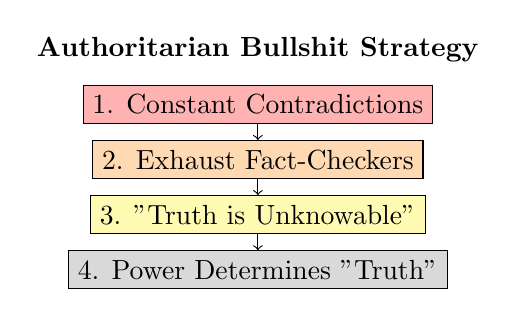
\begin{tikzpicture}[scale=0.7]
			\node at (0,3) {\textbf{Authoritarian Bullshit Strategy}};
			% Step 1
			\node[draw, rectangle, fill=red!30] (step1) at (0,2) {1. Constant Contradictions};
			% Step 2
			\node[draw, rectangle, fill=orange!30] (step2) at (0,1) {2. Exhaust Fact-Checkers};
			% Step 3
			\node[draw, rectangle, fill=yellow!30] (step3) at (0,0) {3. "Truth is Unknowable"};
			% Step 4
			\node[draw, rectangle, fill=gray!30] (step4) at (0,-1) {4. Power Determines "Truth"};
			
			\draw[->] (step1) -- (step2);
			\draw[->] (step2) -- (step3);
			\draw[->] (step3) -- (step4);
		\end{tikzpicture}
	\end{frame}
	
	% Slide 32: Case Study: Alternative Facts and Post-Truth
	\begin{frame}{Case Study: Alternative Facts and Post-Truth}
		\begin{itemize}
			\item The phrase \textbf{"alternative facts"} entered public discourse in 2017, perfectly embodying Frankfurt's concept of indifference to truth.
			\item This wasn't claiming that specific statements were true or false, but that the very concept of objective facts could be dismissed.
			\item The term \textbf{"post-truth"} describes our current era where emotional appeals and tribal loyalty matter more than factual accuracy.
			\item These concepts represent the mainstreaming of bullshit—the open acknowledgment that truth is optional in political discourse.
		\end{itemize}
		
		\begin{example}
			\textbf{Evolution of Political Communication:}
			\begin{itemize}
				\item Traditional lie: "The crowd was 1 million" (knows it was 250,000)
				\item Bullshit: "It was the biggest crowd ever" (doesn't care about actual number)
				\item Post-truth: "Crowd size is whatever we say it is" (rejects measurement itself)
			\end{itemize}
		\end{example}
	\end{frame}
	
	% Slide 33: How Democracies Become Vulnerable
	\begin{frame}{How Democracies Become Vulnerable}
		\begin{itemize}
			\item \textbf{Liberal democracy} depends on citizens sharing enough common facts to have productive disagreements about values and policies.
			\item When bullshit destroys this shared factual foundation, democratic deliberation becomes impossible—we can't debate solutions if we can't agree on problems.
			\item Democratic norms like good-faith argument and compromise assume that participants care about truth, an assumption bullshitters exploit.
			\item Ironically, democracy's protections for free speech make it vulnerable to those who use that freedom to undermine the very possibility of rational discourse.
		\end{itemize}
		
		\begin{alertblock}{The Democratic Dilemma}
			\scriptsize
			Democracy requires:
			\begin{itemize}
				\item Citizens who can evaluate claims rationally
				\item Leaders who engage in good faith
				\item Shared commitment to truth-seeking
			\end{itemize}
			Bullshit destroys all three.
		\end{alertblock}
	\end{frame}
	
	% Slide 34: The Erosion of Shared Reality
	\begin{frame}{The Erosion of Shared Reality}
		\begin{itemize}
			\item Political bullshit creates separate \textbf{information universes} where different groups literally cannot agree on basic facts about what happened.
			\item This goes beyond normal political disagreement—it's not arguing about what policies best serve our values, but about whether events occurred at all.
			\item When each side accuses the other of living in a fantasy world, the concept of objective reality itself becomes politicized.
			\item Without shared reality as a foundation, political violence becomes more likely as groups see opponents not as wrong but as delusional or evil.
		\end{itemize}
		
		\begin{block}{Signs of Eroding Shared Reality}
			\scriptsize
			\begin{tabular}{ll}
				\textbf{Healthy Democracy} & \textbf{Bullshit-Damaged Democracy} \\
				\hline
				"I disagree with your interpretation" & "That never happened" \\
				"Your sources are biased" & "All sources are fake" \\
				"Let's examine the evidence" & "Evidence is a conspiracy" \\
				"We have different values" & "You live in an alternate reality" \\
			\end{tabular}
		\end{block}
	\end{frame}
	
	% Slide 35: Conspiracy Theories as Political Tools
	\begin{frame}{Conspiracy Theories as Political Tools}
		\begin{itemize}
			\item \textbf{Conspiracy theories} represent weaponized bullshit—unfalsifiable narratives that explain everything while proving nothing.
			\item Political actors promote conspiracies not because they believe them but because they're useful for mobilizing supporters and dismissing criticism.
			\item The beauty of conspiracy bullshit is that evidence against the theory becomes evidence of how deep the conspiracy goes.
			\item This creates loyal followers who see the leader as the only source of truth in a world of lies, perfect for authoritarian movements.
		\end{itemize}
		
		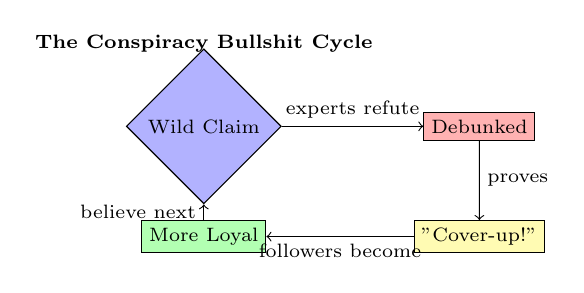
\begin{tikzpicture}[scale=0.7]
			\scriptsize
			\node at (0,3.5) {\textbf{The Conspiracy Bullshit Cycle}};
			\node[draw, diamond, fill=blue!30] (claim) at (0,2) {Wild Claim};
			\node[draw, rectangle, fill=red!30] (debunk) at (5,2) {Debunked};
			\node[draw, rectangle, fill=yellow!30] (deeper) at (5,0) {"Cover-up!"};
			\node[draw, rectangle, fill=green!30] (loyal) at (0,0) {More Loyal};
			
			\draw[->] (claim) -- (debunk) node[midway, above] {experts refute};
			\draw[->] (debunk) -- (deeper) node[midway, right] {proves};
			\draw[->] (deeper) -- (loyal) node[midway, below] {followers become};
			\draw[->] (loyal) -- (claim) node[midway, left] {believe next};
		\end{tikzpicture}
	\end{frame}
	
	% Slide 36: Media Literacy and Democratic Resilience
	\begin{frame}{Media Literacy and Democratic Resilience}
		\begin{itemize}
			\item \textbf{Media literacy} education is essential for democratic survival in an age of sophisticated political bullshit and information warfare.
			\item Citizens need skills to identify reliable sources, recognize manipulation tactics, and understand how their own biases make them vulnerable.
			\item Building \textbf{democratic resilience} means creating institutions and norms that can withstand floods of bullshit without abandoning free speech.
			\item This includes supporting quality journalism, teaching critical thinking in schools, and developing social norms that value truth-seeking over tribal loyalty.
		\end{itemize}
		
		\begin{block}{Building Resilience: Individual and Collective}
			\textbf{Individual}: Develop personal habits of verification and skepticism\\
			\textbf{Community}: Create spaces for good-faith dialogue across differences\\
			\textbf{Institutional}: Support fact-checking and investigative journalism\\
			\textbf{Cultural}: Celebrate truth-seeking over winning arguments
		\end{block}
	\end{frame}
	
	% Slide 37: The Cost of Bullshit to Society
	\begin{frame}{The Cost of Bullshit to Society}
		\begin{itemize}
			\item The \textbf{social costs} of widespread bullshit go far beyond individual false beliefs to corrode the foundations of civilized society.
			\item When bullshit dominates, expertise becomes worthless, scientific progress stalls, and problems go unsolved because we can't agree they exist.
			\item Trust—the invisible infrastructure of modern society—erodes when we assume everyone is bullshitting, making cooperation and commerce difficult.
			\item The ultimate cost is \textbf{civilizational decline}: societies that can't distinguish truth from bullshit can't adapt, learn, or solve collective challenges.
		\end{itemize}
		
		\begin{alertblock}{What We Lose to Bullshit}
			\scriptsize
			\begin{itemize}
				\item Public health (vaccine hesitancy, miracle cures)
				\item Economic stability (market manipulation, fraud)
				\item Social cohesion (polarization, violence)
				\item Human progress (science denial, anti-expertise)
			\end{itemize}
		\end{alertblock}
	\end{frame}
	
	% Slide 38: Building Your Bullshit Detection Toolkit
	\begin{frame}{Building Your Bullshit Detection Toolkit}
		\begin{itemize}
			\item Your personal \textbf{bullshit detection toolkit} combines Frankfurt's philosophical insights with practical skills for navigating modern information environments.
			\item Always ask: "Does this person care whether what they're saying is true?" If not, you've identified a bullshitter.
			\item Develop habits of verification, but also recognize when you're being overwhelmed with claims designed to exhaust your fact-checking capacity.
			\item Remember that fighting bullshit isn't just about personal protection—it's about maintaining the social conditions that make truth-seeking possible.
		\end{itemize}
		
		\begin{example}
			\scriptsize
			\textbf{Your Toolkit Checklist:}
			\begin{enumerate}
				\item \textbf{Philosophical}: Understand Frankfurt's framework
				\item \textbf{Emotional}: Notice when content triggers strong feelings
				\item \textbf{Source evaluation}: Check expertise and motivations
				\item \textbf{Cross-reference}: Verify claims through multiple sources
				\item \textbf{Time investment}: Take 30 seconds before sharing
				\item \textbf{Humility}: Admit when you've spread bullshit
			\end{enumerate}
		\end{example}
	\end{frame}
	
	% Slide 39: The Responsibility of Citizens in a Democracy
	\begin{frame}{The Responsibility of Citizens in a Democracy}
		\begin{itemize}
			\item In a democracy, each citizen bears \textbf{personal responsibility} for maintaining the information ecosystem we all depend on.
			\item This means not just avoiding spreading bullshit ourselves, but actively supporting truth-seeking institutions and calling out bullshit when we see it.
			\item We must resist the temptation to use bullshit for "our side" even when opponents do—the damage to shared reality affects everyone.
			\item Young people especially have the power to shape new norms around truth and bullshit in digital spaces you'll inhabit for decades.
		\end{itemize}
		
		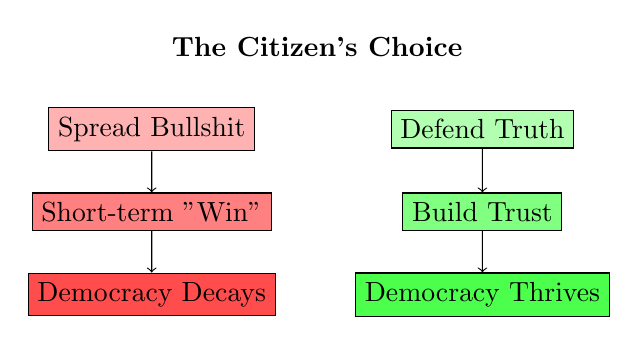
\begin{tikzpicture}[scale=0.7]
			\node at (0,3) {\textbf{The Citizen's Choice}};
			% Path 1
			\node[draw, rectangle, fill=red!30] (bs) at (-3,1.5) {Spread Bullshit};
			\node[draw, rectangle, fill=red!50] (profit) at (-3,0) {Short-term "Win"};
			\node[draw, rectangle, fill=red!70] (decay) at (-3,-1.5) {Democracy Decays};
			
			% Path 2
			\node[draw, rectangle, fill=green!30] (truth) at (3,1.5) {Defend Truth};
			\node[draw, rectangle, fill=green!50] (trust) at (3,0) {Build Trust};
			\node[draw, rectangle, fill=green!70] (thrive) at (3,-1.5) {Democracy Thrives};
			
			\draw[->] (bs) -- (profit);
			\draw[->] (profit) -- (decay);
			\draw[->] (truth) -- (trust);
			\draw[->] (trust) -- (thrive);
		\end{tikzpicture}
	\end{frame}
	
	% Slide 40: Final Thoughts: Truth Still Matters
	\begin{frame}{Final Thoughts: Truth Still Matters}
		\begin{itemize}
			\item Despite the flood of bullshit from social media, AI, and politics, \textbf{truth still matters} because reality doesn't care about our narratives.
			\item Climate change, pandemics, and economic forces operate regardless of what we choose to believe about them—bullshit offers no protection from consequences.
			\item The fact that Frankfurt's essay became a bestseller shows that people hunger for clarity about truth and deception in confusing times.
			\item Your generation will determine whether we rebuild a culture that values truth or surrender to a post-truth world—the choice is yours to make.
		\end{itemize}
		
		\begin{block}{Remember Frankfurt's Core Insight}
			\begin{center}
				\large
				The bullshitter is a greater enemy of truth than the liar,\\
				because the bullshitter attacks the very idea that truth matters.\\
				\vspace{0.5em}
				\textbf{Don't let them win.}
			\end{center}
		\end{block}
	\end{frame}
	
	
\end{document}